\documentclass[a4paper]{article}
\usepackage[utf8x]{inputenc}  % si utf8
\usepackage{graphicx}
\usepackage{verbatim}

\pagestyle{plain}

\title{\textbf{Technical Design Document}\\- \Huge{Incidence} -}
\author{\emph{CHAMBONNET Kevin}\\\emph{GAUTHIER Silvère}\\\emph{MARTINEZ Thierry}\\\emph{MOKHRETAR Amin}}
\date{\today}

\newcommand{\alinea}{\hspace*{0.5cm}}

\begin{document}
  \maketitle
  \newpage
  \tableofcontents

% Liens utiles : 
% https://www.digipen.edu/fileadmin/website_data/gallery/game_websites/NarbacularDrop/documents/narbacular_drop_technical_design_document.pdf

  \newpage
  \part{Project Overview}
    \section{Gestion du projet}
      \subsection{Gestion de l'équipe}
        \alinea Tous les membres se connaissant et étant supposés être capable de travailler en équipe, nous n'avons fait aucune élection de chef de projet.\\
        \alinea Nous avons opté pour travailler de manière collégiale, et ainsi garder une cohésion de groupe sans pour autant avoir de hiérarchie instaurée au sein du groupe, qui pourrait au contraire déservir la réalisation de nos objectifs.\\
        \alinea Chaque membre a donc autant de pouvoir que les autres, et peut donc participer activement au projet, autant lors de la conception que du développement. Toutes les décisions seront prises suivant la majorité lors de votes.\\\\
        \alinea Pour ce qui est des réunions de projets, nous avons convenu avec notre tuteur d'une réunion, allant d'environ trente minutes à une heure, toutes les une à deux semaines, afin de mettre au point l'avancement du projet. En parallèle, tous les membres de notre équipe se retrouvent une fois par semaine afin de discuter des points clés effectués ou à venir, donner lieu aux votes pour les prises de décisions, ou encore, lors de la phase de développement, travailler en collaboration afin d'optimiser notre travail.\\\\
        \alinea Au niveau du travail collaboratif, nous avons mis en place un dépôt sur github, contenant tant la documentation telle que ce rapport que les sources de notre jeu. Par ailleurs, nous mettrons sur ce dépôt uniquement les fichiers sources, les images et les sons, mais en aucun cas les fichiers temporaires ou les exécutables. Un fichier "makefile" sera disponible pour quiconque voudrait compiler le programme chez lui. Les seuls fichiers binaires disponibles seront les PDF de la documentation, pour un soucis de facilité d'accès.

      \subsection{Découpage en tâches}
        \alinea Afin de préparer le développement du jeu, il était nécessaire de séparer les fonctionnalités les unes des autres. Nous avons abouti à ce diagramme, qui résume notre choix de découpage :
        \begin{figure}
          \begin{center}
            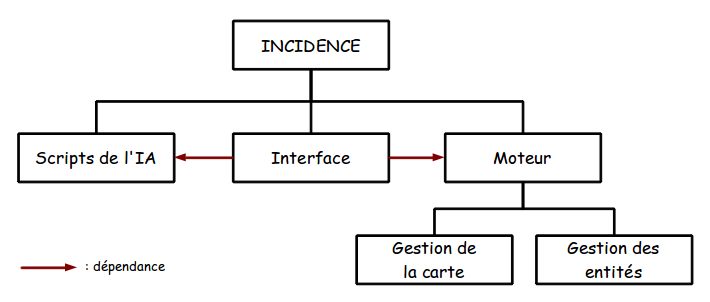
\includegraphics[scale=0.5]{DiagrammeDecoupageProjet.png}
          \end{center}
          \label{DiagDecoupage}
          \caption{Découpage du projet en sous-tâches}
        \end{figure}

      \subsection{Assignation}
        \alinea Le projet étant maintenant découpé en un certain nombre de modules, il ne restait plus qu'à assigner chaque tâche à un ou plusieurs membres de l'équipe. Nous nous sommes organisés comme ceci :
        \begin{itemize}
          \item \textbf{Scripts de l'IA :} MARTINEZ Thierry, MOKHRETAR Amin.
          \item \textbf{Moteur :}
          \begin{itemize}
            \item \textbf{Gestion de la carte :} GAUTHIER Silvère.
            \item \textbf{Gestion des entités :} CHAMBONNET Kevin.
          \end{itemize}
          \item \textbf{Interface :} Tous les membres.
        \end{itemize}
        \alinea Bien entendu, cette répartition n'est pas totalement fixée, elle concerne en réalité l'affectation de responsables de parties, qui seront en charge de celle-ci mais pourront évidemment faire appel aux autres membres pour trouver une solution à un problème par exemple.\\
        \alinea Le détail complet des tâches et assignations se situe dans la section Gestion du temps, page \pageref{GestionTps}.

      \subsection{Gestion du temps}
        \label{GestionTps}
        \alinea Afin de clarifier notre gestion du temps, un diagramme Gantt est disponible dans la documentation de notre projet, et sera mis à jour en fonction de l'avancée du projet.\\
        \alinea Voici tout de même une première estimation du temps nécessaire :
        \begin{figure}
          \begin{center}
            %\includegraphics[scale=0.5]{DiagrammeGantt.png}
          \end{center}
          \label{DiagGantt}
          \caption{Première estimation du temps sous forme de Gantt}
        \end{figure}

    \section{Choix technologiques}
      \subsection{Langages de programmation}
        \alinea Pour des besoins de performances, nous avons comparé différents langages. Pour réduire le temps de recherche et de comparaison, nous nous sommes appuyé sur des tests déjà effectués par d'autre.\\
        \alinea Voici des tests de performances concernant un large panel de langages, comparés ici dans quatre contextes différents :\\
        \begin{figure}
          \begin{center}
            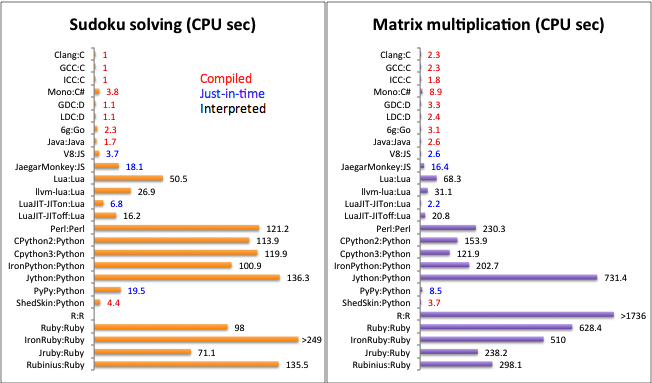
\includegraphics[scale=0.5]{AnalyseLangage1.png}
            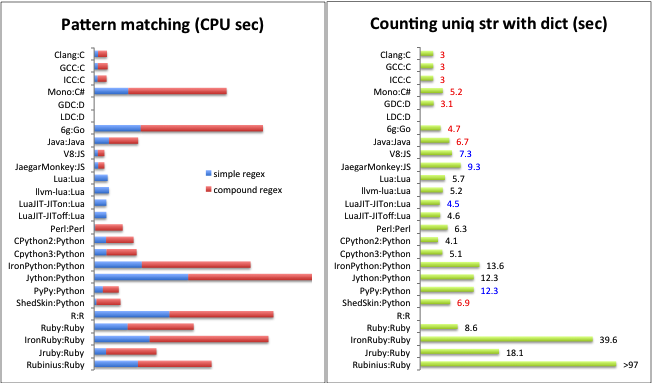
\includegraphics[scale=0.5]{AnalyseLangage2.png} 
          \end{center}
          \label{DiagAnalyse}
          \caption{Comparaisons de performances de divers langages dans des cas donnés}
        \end{figure}
        \alinea Nous pouvons observer que globalement, le langage le plus rapide est ici C++. L'utilisation de ce langage étant très fréquente dans les jeux vidéos, de part sa réputation d'un des langages les plus performants, et tous les membres de notre équipe sachant l'utiliser, nous avons fait le choix de programmer le moteur du jeu en C++.\\
        \alinea Afin d'optimiser encore la rapidité du moteur, nous avons cherché à associer son coeur écrit en C++ avec un langage de scripting qui permettra de mettre en place les différentes actions du jeu.\\ D'après les graphiques ci-dessus, nous avons opté pour le langage LUA, performant et facile d'utilisation (syntaxe proche du C++). En effet, même si Python est très prisé et offre beaucoup plus de possibilités que LUA, nous l'avons estimé bien trop lourd pour l'utilisation que nous allons en faire.\\
        \alinea Les deux langages C++ et LUA sont souvent associés dans les jeux vidéos, notre choix suit donc la tendance, ce qui nous offre une certaine assurance.

      \subsection{Bibliothèques}
        \alinea Pour la gestion graphique des tuiles composant la carte et des différentes entités, nous avons cherché une bibliothèque relativement simple d'utilisation mais surtout performante afin de garder la fluidité gagnée avec le choix des langages de programmation.\\
        \alinea Connaissant la bibliothèque OpenGL, qui est bas niveau et performante dans les affichages deux et trois dimensions, nous nous sommes tournés vers deux bibliothèques utilisant OpenGL : SDL et SFML.\\
        \alinea D'après plusieurs sites web et forums, les dernières versions (respectivement 2.0 et 2.1) de ces deux bibliothèques se valent en terme de performance.\\
        \alinea En confrontant nos préférences personnelles quant au choix de l'une ou l'autre, nous nous sommes finalement mis d'accord pour utiliser la bibliothèque graphique SFML 2.1, qui paraît plus simple d'utilisation que la SDL. De plus, elle permet une gestion aisée des fichiers audio, ce qui sera un plus pour la finalité de notre jeu.

    \section{Profil de risques}
      %Tableau conduite projet
		
\newpage
  \part{Code Overview}
    \section{Format des Fichiers}
      \alinea Le moteur de jeu étant écrit en C++, nous utiliserons des fichiers d'en-tête au format HPP et des fichiers de définition au format CPP. Pour les scripts d'IA des entités, le langage étant Lua, ceux-ci seront au format LUA.\\
      \alinea Toutes les images nécessaires au jeu seront au format PNG afin de pouvoir utiliser la transparence et garder la pleine qualité d'image (contrairement à JPEG qui perd de l'information à la compression).\\
      \alinea Les sons quant à eux seront au format WAV afin d'éviter toute gestion de la compression de fichier pour de petits fichiers qui n'en ont aucunement besoin.

      \subsection{Animation}
        \begin{verbatim}
          Chemin/vers/image.png size_x_sprite size_y_sprite play?(1/0) loop?(1/0)
          +Frame position_x position_y temps_affichage
          +Frame position_x position_y temps_affichage
          +Frame position_x position_y temps_affichage
        \end{verbatim}
      
      \subsection{Tileset}
      
      \subsection{Carte}
      
      \subsection{Sauvegarde}
      
    \section{Commentaires}
      \alinea Chaque fichier aura un en-tête devant contenir une brève explication quant au rôle de celui-ci, ainsi que les date de création et de dernière modification afin de faciliter les éventuelles recherches de versions sur le dépôt distant.\\
      \begin{verbatim}
        /*******************
        ** Description    **
        **                **
        ** Creation :     **
        ** Modif :        **
        *******************/
      \end{verbatim}
      \alinea Si une méthode ou fonction, voir même un bloc, dépasse une certaine taille (environ 10 lignes) ou devient trop compliquée, un commentaire sera ajouté avant celle-ci expliquant brièvement son processus :
      \begin{verbatim}
        /** Description :
        *** Entrée : ...
        *** Sortie : ...
        **/
      \end{verbatim}
      \begin{small}
        \begin{tabular}{| c | c |}
          \hline
          \textbf{Marqueur spécifique} & \textbf{Signification}\\
          \hline
      %En tableau/liste : |Marqueur spécifique|Signification|
          TODO & A mettre à la place du code d'une fonctionnalité à implémenter\\
          \hline
          RECODE & A mettre au dessus du bloc d'une fonctionnalité à refaire\\
          \hline
          FIXME & A mettre au dessus du bloc d'une fonctionnalité contenant un bug\\
          \hline
        \end{tabular}
      \end{small}

    \section{Convention de Nommage}
      \begin{small}
        \begin{tabular}{| c | c |}
          \hline
          \textbf{Type de variable} & \textbf{Format du nom}\\
          \hline
          Classe & Majuscule suivit de minuscules\\
          \hline
          Méthode& Minuscules (pour les mots composés,\\
          et & chaque mots suivant est\\
          Fonction & une majuscule suivit de minuscules)\\
          \hline
          Attribut de classe & m\_\\
          \hline
          Variable globale & g\_\\
          \hline
        \end{tabular}
      \end{small}

    \section{Gestion du code source}
      \alinea Afin de faciliter le travail collaboratif, nous utilisons un dépôt utilisant le gestionnaire de version GIT, hébergé sur le site https://github.com/. Sur ce dépôt seront présents tous les fichiers sources nécessaires au développement du jeu ainsi que les documentations au format Latex et PDF (même si aucun fichier binaire ne devrait être présent, il est plus pratique de récupérer directement un tel fichier que de le compiler soit-même). De plus, y seront stockées toutes les données utilisées par le jeu telles que les images et les sons. Seuls les fichiers temporaires, exécutables et fichiers de sauvegarde ne seront pas stockés.
		
\newpage
  \part{Développement}
    \section{Le Moteur}
      \alinea Le moteur du jeu est très basique et sert surtout à la gestion plus simplifiée des différents états du jeu ainsi que de toutes les ressources.
      
      \subsection{Etat}
        \alinea Le Moteur contient un gestionnaire d'état qui permet de contrôler et d'appeler le dernier état du jeu. Une classe abstraite Etat est la classe mère de tous les états, chaque état ainsi créé aura une méthode de mise à jour, d'affichage et de gestion des différentes actions clavier/souris du joueur.
        
      \subsection{Animation}
        \alinea Une classe Animation a été créée pour faciliter la création et le contrôle de toutes les animations du jeu. Toutes les animations peuvent être modifiées grâce aux fichiers d'initialisation de chacune.
        
      \subsection{Gestion des Ressources}
        \alinea Une classe de gestionnaire de ressources permet de gérer toutes les ressources du jeu pour éviter de charger en double ou plus certaines ressources. Ce gestionnaire gère toutes les textures, images et sons.

    \section{Les Entités}
      \alinea Les entités constitueront tout ce qu'il y a de mobile dans le monde : les Citoyens et les différents Animaux.\\
      Chaque entité possèdera des méthodes communes utilisées dans les différents scripts de leur IA :
      \begin{itemize}
        \item \textbf{Connaître sa position sur la carte : } La position sera donnée en valeur entière correspondant à la case sur laquelle l'entité est présente.
        \item \textbf{Se déplacer vers une direction donnée : } L'entité se déplacera en ligne droite dans cette direction. Si des obstacles se trouvent sur le chemin, elle essayera, si possible, de les contourner.
        \item \textbf{Connaître les entités alentour : } Recupère une liste d'entités présentes dans le champ de vision de l'entité appelant la méthode.
        \item \textbf{Connaître les cases alentour : } Recupère une listes de booléen correspondants aux différentes cases présentes dans le champ de vision, avec pour valeur TRUE si la case est franchissable, FALSE sinon.
      \end{itemize}
      \alinea De plus, toutes les entités auront une méthode de mise à jour, qui appellera le script en cours, et une d'affichage, pour l'afficher sur la carte.
      \alinea Chaque entité possèdera aussi une liste d'attributs modifiables par les différentes méthodes : 
      \begin{itemize}
        \item \textbf{Sa position sur la carte : } En pixel et non en case.
        \item \textbf{Son activité : } C'est-à-dire, le script en cours.
        \item \textbf{Son Animation en cours : } Le visuel de l'entité.
      \end{itemize}
      
      \subsection{Les citoyens}
        \alinea Les Citoyens sont les entités que le joueur devra garder en vie et c'est eux qui auront un impact direct sur l'environnement.
        Pour cela, ils possèdent des méthodes supplémentaires :
        \begin{itemize}
          \item \textbf{Connaître les positions d'un type de case alentour : } Retourne une liste de positions correspondantes aux positions d'un type de case, passé en paramètre, dans le champ de vision du citoyen.
          \item \textbf{Interagir avec une case : } Le citoyen interagit avec la case passée en paramètre. Ex.: Pour un arbre, il le coupera.
        \end{itemize}
        \alinea Chacun des citoyens aura un métier assigné durant la nuit, et c'est ce métier qui définira le groupe de scripts que le citoyen suivra pour effectuer ses actions. Ce métier ajoute donc aussi de nouveaux attributs :
        \begin{itemize}
          \item \textbf{Le nom du métier : } Pour facilement connaître le métier mais aussi la ressource associée à celui-ci et surtout le groupe de scripts à appeler.
          \item \textbf{La quantité de ressources portée : } Chaque entité pouvant porter qu'un seul type de ressource, cette quantité est associée à la ressource, elle-même liée au métier. Ex.: Bois pour un Bûcheron.
        \end{itemize}
        
      \subsection{Liste des scripts}
      
    \section{La Carte}
      \subsection{Les Tuiles}
      
      \subsection{Le Tileset}
      
      
\newpage
  \part{Milestones}
    12 Mars 2013 : Gestion de la carte et des entités terminée + ajout des entités sur la carte + ajout des scripts aux entités\\
    19 Mars 2013 : Finalisation des scripts et des entités\\
    10 Avril 2013 : Fin de la première version :D\\
      
      
\newpage
  \part{Effets Graphiques}
    
      
\newpage
  \part{Effets Sonores}

\end{document}
